%% abtex2-modelo-trabalho-academico.tex, v-1.7.1 laurocesar
%% Copyright 2012-2013 by abnTeX2 group at http://abntex2.googlecode.com/
%%
%% This work may be distributed and/or modified under the
%% conditions of the LaTeX Project Public License, either version 1.3
%% of this license or (at your option) any later version.
%% The latest version of this license is in
%%   http://www.latex-project.org/lppl.txt
%% and version 1.3 or later is part of all distributions of LaTeX
%% version 2005/12/01 or later.
%%
%% This work has the LPPL maintenance status `maintained'.
%%
%% The Current Maintainer of this work is the abnTeX2 team, led
%% by Lauro C\'{e}sar Araujo. Further information are available on
%% http://abntex2.googlecode.com/
%%
%% This work consists of the files abntex2-modelo-trabalho-academico.tex,
%% abntex2-modelo-include-comandos and abntex2-modelo-references.bib
%%

% ------------------------------------------------------------------------
% ------------------------------------------------------------------------
% abnTeX2: Modelo de Trabalho Academico (tese de doutorado, dissertacao de
% mestrado e trabalhos monograficos em geral) em conformidade com
% ABNT NBR 14724:2011: Informacao e documentacao - Trabalhos academicos -
% Apresentacao
% ------------------------------------------------------------------------
% ------------------------------------------------------------------------

%ARQUIVO DE PREAMBULO DA TESE - PACOTES E CONFIGURA\c{C}\~{O}ES

\documentclass[
	% -- op\c{c}\~{o}es da classe memoir --
	12pt,				% tamanho da fonte
	openright,			% cap\'{\i}tulos come\c{c}am em p\'{a}g \'{\i}mpar (insere p\'{a}gina vazia caso preciso)
	oneside,			% para impress\~{a}o em verso e anverso. Oposto a oneside
	a4paper,		% tamanho do papel.
	% -- op\c{c}\~{o}es da classe abntex2 --
	%chapter=TITLE,		% t\'{\i}tulos de cap\'{\i}tulos convertidos em letras mai\'{u}sculas
	%section=TITLE,		% t\'{\i}tulos de se\c{c}\~{o}es convertidos em letras mai\'{u}sculas
	%subsection=TITLE,	% t\'{\i}tulos de subse\c{c}\~{o}es convertidos em letras mai\'{u}sculas
	%subsubsection=TITLE,% t\'{\i}tulos de subsubse\c{c}\~{o}es convertidos em letras mai\'{u}sculas
	% -- op\c{c}\~{o}es do pacote babel --
	english,			% idioma adicional para hifeniza\c{c}\~{a}o
	%french,			% idioma adicional para hifeniza\c{c}\~{a}o
	%spanish,			% idioma adicional para hifeniza\c{c}\~{a}o
	brazil,				% o \'{u}ltimo idioma \'{e} o principal do documento
	sumario=tradicional,
	]{abntex2}

% ---
% PACOTES
% ---

% ---
% Pacotes fundamentais
% ---
\usepackage{cmap}				        % Mapear caracteres especiais no PDF
\usepackage{lmodern}			      % Usa a fonte Latin Modern			
\usepackage[T1]{fontenc}		    % Selecao de codigos de fonte.
\usepackage[utf8]{inputenc}		  % Codificacao do documento (convers\~{a}o autom\'{a}tica dos acentos)
\usepackage{lastpage}			      % Usado pela Ficha catalogr\'{a}fica
\usepackage{indentfirst}		    % Indenta o primeiro par\'{a}grafo de cada se\c{c}\~{a}o.
\usepackage{color}				      % Controle das cores
\usepackage[pdftex]{graphicx}	  % Inclus\~{a}o de gr\'{a}ficos
\usepackage{epstopdf}           % Pacote que converte as figuras em eps para pdf
\usepackage{lipsum}             % Pacote que gera texto dummy
\usepackage{blindtext}          % Pacote que gera texto dummy
% ---
		
% ---
% Pacotes adicionais, usados apenas no \^{a}mbito do Modelo Can\^{o}nico do abnteX2
% ---
%\usepackage{nomencl}

\let\printglossary\relax
\let\theglossary\relax
\let\endtheglossary\relax

\usepackage[nonumberlist]{glossaries} % nonnumberlist nao mostra as paginas nas quais os acronimos aparecem no texto
\usepackage{amsmath}
\usepackage{amssymb}
\usepackage{bbm}
\usepackage[chapter]{algorithm}
\usepackage{algorithmic}
\usepackage{multirow}
\usepackage{rotating}
\usepackage{pdfpages}
\usepackage{subfig}
\usepackage{booktabs}
\usepackage{pdflscape}
\usepackage{chngcntr}
\counterwithin{figure}{chapter}
\counterwithin{table}{chapter}

% ---
% Pacotes de cita\c{c}\~{o}es
% ---
\usepackage[brazilian,hyperpageref]{backref}	 % Paginas com as cita\c{c}\~{o}es na bibl
\usepackage[alf,abnt-etal-cite=2,abnt-etal-list=0,abnt-etal-text=emph]{abntex2cite}	% Cita\c{c}\~{o}es padr\~{a}o ABNT
% ---
% Pacote de customiza\c{c}\~{a}o - Unicamp
% ---
\usepackage{unicamp}
% ---
% CONFIGURA\c{C}\~{O}ES DE PACOTES
% ---

% ---
% Configura\c{c}\~{o}es do pacote backref
% Usado sem a op\c{c}\~{a}o hyperpageref de backref
\graphicspath{{eps/}}
\DeclareGraphicsExtensions{.eps}

%customiza\c{c}\~{a}o do negrito em ambientes matem\'{a}ticos
\newcommand{\mb}[1]{\mathbf{#1}}
\newcommand{\abs}[1]{\left|#1\right|}
\newcommand{\norm}[1]{\left\|#1\right\|}
\newcommand{\partialorder}{\cdot \geq}
\newcommand{\h}{\mathrm{h}}
\newcommand{\x}{\mathrm{x}}
\newcommand{\z}{\mathrm{z}}
\newcommand{\entropia}[1]{H{(#1)}}
%customiza\c{c}\~{a}o de teoremas
\newtheorem{mydef}{Defini\c{c}\~{a}o}[chapter]
\newtheorem{lemm}{Lema}[chapter]
\newtheorem{theorem}{Teorema}[chapter]
\floatname{algorithm}{Pseudoc\'{o}digo}
\renewcommand{\listalgorithmname}{Lista de Pseudoc\'{o}digos}
\newenvironment{proof}[1][Prova]{\begin{trivlist}
\item[\hskip \labelsep {\bfseries #1}]}{\end{trivlist}}
\newcommand{\qed}{\hfill \ensuremath{\Box}}

\renewcommand{\backrefpagesname}{Citado na(s) p\'{a}gina(s):~}
% Texto padr\~{a}o antes do n\'{u}mero das p\'{a}ginas
\renewcommand{\backref}{}
% Define os textos da cita\c{c}\~{a}o
\renewcommand*{\backrefalt}[4]{
	\ifcase #1 %
		Nenhuma cita\c{c}\~{a}o no texto.%
	\or
		Citado na p\'{a}gina #2.%
	\else
		Citado #1 vezes nas p\'{a}ginas #2.%
	\fi}%
% ---


% ---
% Configura\c{c}\~{o}es de apar\^{e}ncia do PDF final

% alterando o aspecto da cor azul
\definecolor{blue}{RGB}{41,5,195}

% informa\c{c}\~{o}es do PDF
\makeatletter
\hypersetup{
     	%pagebackref=true,
		pdftitle={\@title},
		pdfauthor={\@author},
    pdfsubject={\imprimirpreambulo},
	  pdfcreator={LaTeX with abnTeX2},
		pdfkeywords={abnt}{latex}{abntex}{abntex2}{trabalho acad\^{e}mico},
		hidelinks,					% desabilita as bordas dos links
		colorlinks=false,       	% false: boxed links; true: colored links
    linkcolor=blue,          	% color of internal links
    citecolor=blue,        		% color of links to bibliography
    filecolor=magenta,      	% color of file links
		urlcolor=blue,
%		linkbordercolor={1 1 1},	% set to white
		bookmarksdepth=4
}
\makeatother
% ---

% ---
% Altera as margens padrões
% ---
\setlrmarginsandblock{3cm}{2cm}{*}
\setulmarginsandblock{3cm}{2cm}{*}
\checkandfixthelayout
% ---

% ---
% Espa\c{c}amentos entre linhas e par\'{a}grafos
% ---
\linespread{1.3}

% O tamanho do par\'{a}grafo \'{e} dado por:
\setlength{\parindent}{2.0cm}

% Controle do espa\c{c}amento entre um par\'{a}grafo e outro:
\setlength{\parskip}{0.2cm}  % tente tamb\'{e}m \onelineskip

% ---
% Informacoes de dados para CAPA e FOLHA DE ROSTO
% ---
\titulo{Desenvolvimento de um rastreador estrelar para determinação de atitude de cubsat}
\autor{Hebert Wandick Parreira}
\local{Campinas}
\data{2022}
\orientador{Rodrigo Moreira Bacurau}
\coorientador[Co-orientador]{Prof. Dr. Co-orientador}
\instituicao{%
    UNIVERSIDADE ESTADUAL DE CAMPINAS
    \par
    Faculdade de Engenharia Mecanica	
    }
\tipotrabalho{Trabalho de conslução de curso}
%% O preambulo deve conter o tipo do trabalho, o objetivo, o nome da institui\c{c}\~{a}o e a \'{a}rea de concentra\c{c}\~{a}o
\preambulo{Trabalho apresentado \`{a} Faculdade de Engenharia Mecanica da Universidade Estadual de Campinas como parte dos requisitos exigidos para a obten\c{c}\~{a}o do t\'{\i}tulo de Engenheiro de Controle e automação.}
%\tipotrabalho{Disserta\c{c}\~{a}o (Mestrado)}
%\preambulo{Disserta\c{c}\~{a}o apresentada \`{a} Faculdade de Engenharia El\'{e}trica e de Computa\c{c}\~{a}o da Universidade Estadual de Campinas como parte dos requisitos exigidos para a obten\c{c}\~{a}o do t\'{\i}tulo de Mestre em Engenharia El\'{e}trica, na \'{A}rea de xxx.}
% --- 

% ---- compila o \'{\i}ndice  ----
\makeindex
%\makeglossaries
% ---
\usepackage[utf8]{inputenc}

% Required package
\usepackage{amsmath,bm}

% ---- In\'{\i}cio do documento ----
\begin{document}

% Retira espa\c{c}o extra obsoleto entre as frases.
\frenchspacing

% ---- ELEMENTOS PR\'{E}-TEXTUAIS ----
%\pretextual

% --- Capa ---
\imprimircapa
% ---

% --- Folha de rosto (o * indica que haver\'{a} a ficha catalogr\'{a}fica) ---
\imprimirfolhaderosto
% ---

% --- Inserir a ficha catalogr\'{a}fica ---
%\includepdf{ficha_catalografica.pdf}

% --- Para a vers\~{a}o final, delete as linhas abaixo e insira a linha do \includepdf
 %\begin{fichacatalografica}
 %   \vspace*{\fill}
 %   \begin{center}
 %       \textsc{Inclua aqui o pdf com a ficha catalogr\'{a}fica fornecida pela BAE.}
 %   \end{center}
 %   \vspace*{\fill}
% --- --- ---
    %\includepdf{ficha-catalografica.pdf}
 %\end{fichacatalografica}
% ---

% ---

% --- Inserir folha de aprova\c{c}\~{a}o ---
%\includepdf{folha_de_assinaturas_oficial.pdf}

% Isto \'{e} um exemplo de Folha de aprova\c{c}\~{a}o, elemento obrigat\'{o}rio da NBR
% 14724/2011 (se\c{c}\~{a}o 4.2.1.3). Voc\^{e} pode utilizar este modelo at\'{e} a aprova\c{c}\~{a}o
% do trabalho. Ap\'{o}s isso, substitua todo o conte\'{u}do deste arquivo por uma
% imagem da p\'{a}gina assinada pela banca com o comando abaixo:

% --- Na vers\~{a}o final, exclua essas linhas e insira o \includepdf
%\newpage
%\vspace*{\fill}
%\begin{center}
%    \textsc{Inclua aqui a folha de assinaturas.}
%\end{center}
%\vspace*{\fill}
%\newpage
% --- --- ---
%\includepdf[pagecommand={\thispagestyle{plain}}]{folha-assinaturas.pdf}	
\cleardoublepage

% ---

%% --- Dedicat\'{o}ria ---
%\include{Dedicatoria}
%% ---

%% --- Agradecimentos ---
%\begin{agradecimentos}
%	Escreva seus agradecimentos.
    
    
%	\lipsum[1-3]
%\end{agradecimentos}

%% --- RESUMOS (em portugu\^{e}s e ingl\^{e}s --- 150 a 500 palavras

\begin{resumo}
    
    O bjetivo deste trabalho é realizar o desenvolvimento de um sistema de rastreamento estrelar, com baixo custo, baixo consumo de energia e com volume mássico e peso reduzido.
    Estas restrições e objetivos  se devem a aplicação desejada ao sistema, que será utilizado em cubesats.

    Para a realização deste objetivo, foi realizada uma ampla pesquisa na literatura científica acadêmica a respeito do assunto em questão, além disso foi utilizado um conjunto de técnicas e ferramentas de programação para garantir a qualidade do sistema final.
    
    Os resultados do trabalho estão divididos em duas partes, com a primeira constituindo um simulador estrelar e a segunda sendo o sistema de rastreamento estrelar em si. A primeira parte foi desenvolvida para auxiliar no desenvolvimento e averiguar a acurácia do sistema de rastreamento estrelar em ambiente simulado.
    
    \vspace{\onelineskip}

    \noindent\textbf{Palavras-chaves}: rastreador estrelar; cubesat; determinador de atitude.

    \vspace{\onelineskip}
    \vspace{\onelineskip}

    \begin{otherlanguage*}{english}
    \begin{center}{\ABNTEXchapterfont\huge Abstract}\end{center}

Same content of "Resumo".       

    \vspace{\onelineskip}

    \noindent\textbf{Keywords}: keyword 1; keyword 2; keyword 3. 

    \end{otherlanguage*}
\end{resumo}
%% ---



%% ---
%
%% --- Ep\'{\i}grafe  ---
%\begin{epigrafe}
%    \vspace*{\fill}
%	\begin{flushright}
%		\textit{``Escreva aqui a sua ep\'{\i}grafe''\\
%		(Cita\c{c}\~{a}o)}
%	\end{flushright}
%\end{epigrafe}
%% ---
%
%
%% --- inserir lista de ilustra\c{c}\~{o}es ---
\pdfbookmark[0]{\listfigurename}{lof}
\listoffigures*
\cleardoublepage
%% ---
%
%% --- inserir lista de tabelas ---
\pdfbookmark[0]{\listtablename}{lot}
\listoftables*
\cleardoublepage
%% ---
%
%% --- inserir lista de Acronimos e Abrevia\c{c}\~{o}es ---
%\renewcommand{\nomname}{Lista de Acr\^{o}nimos e Abrevia\c{c}\~{o}es}
%\pdfbookmark[0]{\nomname}{las}
%\printnomenclature
%\cleardoublepage
%% ---

%% --- inserir o sumario ---
\pdfbookmark[0]{\contentsname}{toc}
\tableofcontents*
\clearpage
%% ---

\pagenumbering{arabic}
\setcounter{page}{14}

% ---- ELEMENTOS TEXTUAIS ----
\textual


\chapter{Introdução}
\label{cap:Introducao_init}

Este documento apresenta o Trabalho de Graduação do aluno Hebert Wandick Parreira, que é realizado sob a orientação do Professor Dr. Rodrigo Moreira Bacurau, no curso de Engenharia de Controle e Automação do nível da graduação na Faculdade de Engenharia Mecânica da UNICAMP.

Um dos principais sistemas de um satélite é o sistema de determinação de atitude, o qual é parte do sistema de controle de atitude de um cubesat, que é responsável pela orientação espacial do satélite. Este sistema é de extrema importância, pois os cubesats podem possuir missões nas quais a orientação angular fixa é necessária ou uma variação angular controlada seja necessária, como para tirar fotos da superfície terrestre e fornecer acesso de rede a estação fixa em solo, como por exemplo, é o caso do Starlink.

Durante este projeto, será desenvolvido sistema de rastreamento estrelar para cubesat, com aplicabilidade  na indústria aeroespacial. O sistema será baseado em visão computacional. Pretende-se utilizar webcams convencionais e utilizar como unidade de processamento embarcados de baixo custo que executam Linux, como por exemplo a Raspberry Pi 4.

O foco desse projeto será no desenvolvimento dos algoritmos responsáveis por fazer a captura e análise das imagens, e determinar a posição  angular do cubesat. Para testar o sistema, será desenvolvido uma simulação. Ela consistirá de um monitor juntamente de um software  de simulação do céu estrelado a ser visualizado pelo dispositivo. 

Essa simulação, será desenvolvida em linguagem Python e permitirá a rotação em todo o espaço com 360 graus de liberdade em todos os eixos, por fim será realizada uma validação final com uma webcam.

\section{Motivação}
\label{sec:Introducao_motivacao}
Com o desenvolvimento da eletrônica, os circuitos e sistemas presentes em satélites conseguiram se tornar menores, mais leves, mais baratos, rápidos, e com maior eficiência  energética. Além disso, o desenvolvimento de uma padronização nas dimensões destes pequenos satélites possibilitou um decréscimo ainda maior de custo.

Em universidades e StartUps o estudo e desenvolvimento de cubesats vem crescendo rapidamente, mesmo que os pequenos satélites apresentem limitações físicas e energéticas, o custo benefício em sua aplicabilidade é grande.

Outra limitação está na capacidade do satélite de se localizar e orientar no espaço, ou seja, controlar a sua atitude, que devido às restrições já mencionadas, costumam ser extremamente limitados ou mesmo inexistentes ~\cite[]{Diaz}. Com isto, as possibilidades de aplicações destes cubesats tornam-se consideravelmente limitadas.

A primeira etapa para realizarmos o controle de atitude, é identificar de forma confiável, precisa e contínua a atitude do satélite ~\cite[]{Diaz}. No espaço existem pontos de referência que podem ser utilizados para a determinação da atitude, como o Sol, Lua e a Terra, porém estas referências não são consistentes, já que o Sol pode estar encoberto, e a análise da superfície terrestre vista do espaço varia muito, devido a nuvens e outros fenômenos meteorológicos. Além disso, a análise de imagens complexas é custosa computacionalmente, o que devido às limitações de volume e energia, tornam a aplicação extremamente complicada.

Outra opção é utilizar o campo magnético da terra, porém a interferência eletromagnética é algo relativamente comum, uma vez que os próprios circuitos elétricos do satélite podem gerar interferências.

Uma terceira opção é a utilização de uma câmera realizando a análise das estrelas, o fato do satélite estar no espaço faz com que as estrelas estejam na maioria do tempo no campo de visão do satélite ~\cite[]{Tappe}.

Realizar o controle de atitude apenas utilizando IMU (Inertial measurement unit)  é difícil, pois IMU são suscetíveis a erros de desvio de Offset, erros de Instabilidade, temperatura, são sensíveis a pancadas e vibrações ~\cite[]{Young}. Desta forma utiliza-se IMUs de alto custo, que são caros, e em sua maioria, grandes. 

Com a utilização de um dos três métodos de sensorialmente apresentados anteriormente, pode-se utilizar IMUs de menor custo para auxiliar o processo, e fazer fusão sensorial, pois a deriva dos giroscópios, causará erros de orientações consideráveis em poucos segundos se não houver algum outro sistema para identificação de atitude.

Devido a questões de custo e disponibilidade, utiliza-se componentes de prateleira (sensores e chips já prontos e vendidos em massa). Geralmente fazendo uso da tecnologia MEMS (micro electro mechanical systems), os quais são relativamente baratos, pequenos e possuem massa reduzida. 



%\section{Determinação da Atitude}
%\label{sec:sec01}
%Atitude de um satélite consiste em sua orientação no espaço, um satélite possui 6 graus de liberdade, (três de rotação e três de translação)  normalmente  modelados em 12 variáveis de estado: 6 variáveis de posição e 6 de suas respectivas derivadas, já que a estabilização e o controle de orientação são normalmente desejados no controle ~\cite[]{Souza}.

%Do Cálculo sabemos, que a derivada da posição a sua velocidade, e sabendo-se o valor da posição a todo instante pode-se calcular a derivada, portanto é possível facilmente obter a informação da velocidade. Desta forma, é necessário apenas a utilização de sensores de posição, o que é verdade, porém a precisão se eleva muito ao utilizarmos múltiplos sensores, e realizarmos uma fusão sensorial completa. 

%Este trabalho foca no desenvolvimento do rastreador estelar que é responsável pela determinação da rotação nos 3 eixos, já pensado para a incorporação em tais conjuntos de dados futuramente.



%\include{star_trackers/tar_trackers.tex}

%\chapter{Simulação}
\section{Objetivo}

O objetivo da simulação é poder realizar teste em ambiente controlado, de forma a se averiguar a precisão, acurácia e velocidade de processamento da posição por parte do Star Tracker. Para isto, a simulação deve implementar modelos matemáticos que representem o sistema real o mais fielmente possível.

\section{Recursos e características}

\textbf{GUI (Graphical User Interface):} A simulação é inteiramente controlada através de uma GUI criada para facilitar o controle e a execução dos testes, também é utilizada para facilitar a visualização e a correção de possíveis erros e bugs no software e no desenvolvimento do trabalho em geral. A implementação dos módulos de funcionamento do software segue conceitos dos TDD (Test driven  development), juntamente da arquitetura de software MVC (model view controller), para organizar o funcionamento da interface em si.

\textbf{Gerador de campo de visão:} Esta é a função principal do software de simulação, que é gerar uma janela com o campo de visão que teoricamente seria visto pela câmera, a imagem gerada é monocromática com as estrelas projetadas sobre a superfície plana do monitor, neste trabalho as estrelas simuladas são apenas círculos brancos em um fundo preto, porém são estrelas retiradas de uma base de dados reais.

\textbf{Load de arquivos:} Para facilitar a mudança de parâmetros durante os testes e simulações , o software carrega todas as informações inerentes a configuração e execução dos testes, através de caixas de diálogo que pedem a seleção dos arquivos de simulação. Para uma maior modularidade, cada informação está dividida em arquivos diferentes, com arquivos separados para configuração de câmera, base de dados de estrelas e sequência de movimentos a ser realizada.

\textbf{Elementos auxiliares de visualização:} Além das funcionalidades básicas, o software implementa  recursos de configuração  de aspectos visuais. Apesar de não serem estritamente necessários são de extrema importância  para análises menos rigorosas das informações, como por exemplo, o plot 3D, a projeção cartográfica em 2D. Com opções de visualização da posição das câmeras e demais auxílios.

\textbf{Controles manuais e automáticos:} O software possui controles manuais de rotação, que permitem a rotação da simulação em todos os 3 eixos de liberdade, através de configurações na GUI, além disto o usuário pode preparar uma sequência de movimentos e suas respectivas durações previamente.

\textbf{Salvar frames:} O usuário pode salvar frames de imagem em arquivos png para facilitar a utilização posterior da posição.

\section{Projeção em perspectiva}

A projeção descreve matemática como representar um ponto com 3 graus de liberdade, no espaço bidimensional do monitor e do frame da câmera. Essa transformação pode ser realizada através de matrizes, que levam em consideração elementos como o ângulo focal da lente, a resolução e proporção da imagem.

\subsection{Square Frustum}

Frustum retangular é um espaço que contém a linha de visão de  um visualizador como se este possuísse um ângulo de visão retangular, que é caso de câmeras com CCD retangulares, para melhor entender este conceito recomenda-se a observação da Figura \ref{fig:frustum}.

\begin{figure}[h]
    \centering
    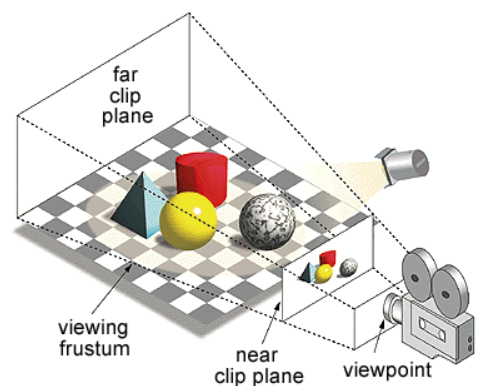
\includegraphics[width=0.5\textwidth]{images/frustum.png}
    \caption{Visualização Frustum rectangular, Fonte: ~\cite[]{the_free_dictionary}}
    \label{fig:frustum}
\end{figure}

A existência de um plano ao fundo na cena (far clip), se deve ao equacionamento que leva os pontos presentes na cena 3D para o frame 2D da câmara, além de reduzir o custo de processamento requerido pelo programa para gerar a cena sendo parte importante do equacionamento do frame da câmera.

Considerando que o ângulo de visão da câmera esteja apontada para o positivo do eixo x como é mostrado na figura \ref{fig:posicao_inicial_camera}.

\begin{figure}[h]
    \centering
    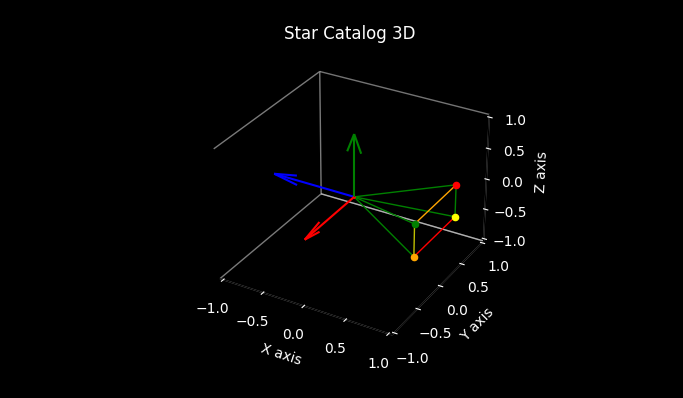
\includegraphics[width=0.5\textwidth]{images/posicao_inicial_camera.png}
    \caption{Visualização da câmera na posição inicial}
    \label{fig:posicao_inicial_camera}
\end{figure}

As setas coloridas presentes na imagem são as coordenadas do frame da câmera, que seguem um esquema de cores usual para esse tipo de aplicação, na figura 17 é demonstrado as relações X,Y e Z com as cores:



\begin{figure}[h]
    \centering
    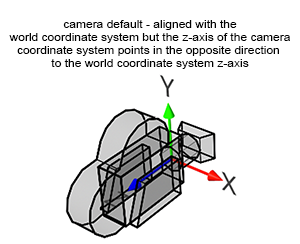
\includegraphics[width=0.5\textwidth]{images/coordenadas.png}
    \caption{Coordenadas do frame da camera. Fonte: ~\cite[]{the_free_dictionary}}
    \label{fig:coordenadas}
\end{figure}


Com isso se desenvolveu a seguinte equação matricial da câmera, seguindo os passos mostrados por Brendan Galea em seu video ~\cite[]{Galea}:

\begin{equation}
    \begin{bmatrix}
        x' \\
        y' \\
        z' \\
        w
    \end{bmatrix}
    =
    \begin{bmatrix}
        \frac{f+n}{f-n} & 0                                 & 0                               & \frac{-2fn}{f-n} \\
        0               & \frac{h}{w*tan(\frac{\theta}{2})} & 0                               & 0                \\
        0               & 0                                 & \frac{1}{tan(\frac{\theta}{2})} & 0                \\
        1               & 0                                 & 0                               & 0
    \end{bmatrix}
    \begin{bmatrix}
        x \\
        y \\
        z \\
        1
    \end{bmatrix}
\end{equation}

Em que, \textbf{f} é a distância do far plane ao ponto (0,0,0), que neste caso é sempre unitário já que a estrelas estão presentes em um círculo unitário, $\Theta$ é o ângulo de abertura  da câmera, \textbf{w} é a quantidade de pixels na horizontal camera, \textbf{h} é quatidade e pixel na vertical da câmera por fim \textbf{n} é a distância do near plane, que neste caso é o coseno de $\frac{\Theta}{2}$.

Nota-se que a matriz de transformação da câmera é uma matriz 4X4 isso ocorre pois as equações de transformação são realizadas através de coordenadas homogêneas e não coordenadas cartesianas tradicionais.

Além da matriz, existe uma equação de clipping que determina se uma estrela deve ou não aparecer no frame, devido a simplicidade da simulação aqui implementada essa equação se tornou apenas um cheque se a estrela se encontrava na metade da esfera celeste em que x é positivo.

O resultado dessa simulação pode ser visto na Figura \ref{fig:resultado_simulacao}.

\begin{figure}[h]
    \centering
    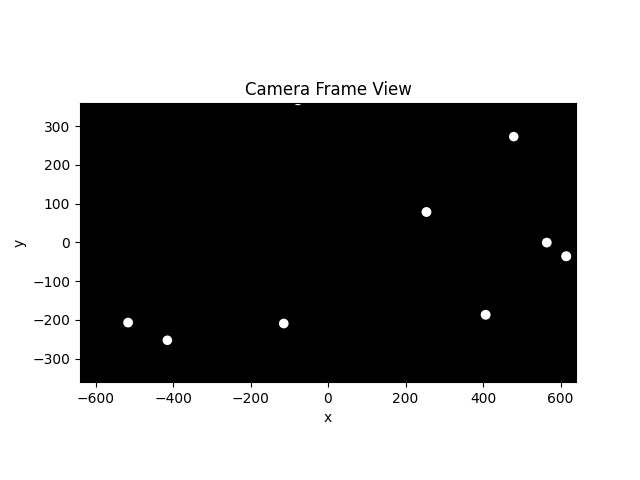
\includegraphics[width=\textwidth]{images/resultado_simulacao.png}
    \caption{Camera frame at position,declination 0º, arcensão 0º, roll 0º}
    \label{fig:resultado_simulacao}
\end{figure}

%\include{rotacao.tex}

%\section{Desenvolvimento de software}

\subsection{Test Driven Development(TDD)}

O  Desenvolvimento Orientado a Testes,  consiste em desenvolver testes separados para cada parte de um software como é o caso das funções, os testes devem garantir que o código funcione e cumpra a tarefa desejada.

Para aplicá-lo, primeiro cria-se o teste ,dessa forma garante-se que o que durante o desenvolvimento do código o resultado inicialmente esperado seja obtido, dessa forma o teste falha na primeira vez que é executado, já que este está testando o recurso que ainda não existe, em seguida é desenvolvido o recurso de forma a fazer o teste passar, então repete-se este ciclo função por função. 

Caso seja localizado um bug no software, primeiramente o desenvolvedor deve implementar um teste que consiga replicar o erro em específico, só então a realizar a correção, dessa forma se garante a correta implementação da solução, assim como o novo software deve manter-se passando nos testes anteriores. Algumas das vantagem de tal método são:
\begin{itemize}
    \item Facilidade em focar em problemas específicos de desenvolvimento
    \item Códigos são fáceis de refatorar
    \item Facilidade em corrigir bugs, mesmo durante o desenvolvimento
    \item Capacidade em garantir do que está funcionando e como está funcionando
    \item Dividir de forma mais clara cada parte do código 
    \item Descobrir falhas de forma prematura durante o processo de desenvolvimento
    \item Maior organização de código
\end{itemize}

Como este projeto é desenvolvido em python, é utilizado o framework pytest, para implementação dos testes, ressalta-se também que apenas os módulos do software responsáveis por realizar a matemática aqui aplicada e desenvolvida, que foram testados por tal metodologia, com a parte do software relacionada a interfaces gráficas não sendo desenvolvidas dessa forma, isto ocorre pois apesar de ser perfeitamente possível de se utilizar TDD, a criação de testes para tais componentes de software costuma ser lenta e difícil, optando-se então por apenas realizar checks visuais neste caso.

\subsection{Model View Controller (MVC)}
MVC é um arquitetura de software desenvolvida para otimizar o processo de desenvolvimento de interfaces gráficas, com foco em diminuir o tempo de manutenção do código, facilitando o debug de elementos visuais do sistema, também facilita a interação de múltiplos desenvolvedores e proporciona uma maior clareza de código exigindo um baixo nível de acoplamento entre as partes. 

Para isso o MVC se divide em 3 componentes principais, o model, o controller e o view, as regras de negócio estão contidas no model assim como as informações  necessárias para execução do programa o controller realizar a interface entre o model e view, que contém as especificações de como os usuários interagem com o sistema.

O view decide como apresentar as informações e como os inputs de informações são feitos, por exemplo o usuário ao clicar em um botão que tem sua aparência e posição especificados pelo view, gera um evento que é tratado pelo controlador que se preciso for irá formatar os dados gerados pela interface então transfere o dado para o model, que executa a aplicação em si, como por exemplo realizando equações matemáticas, carregando arquivos e demais lógicas de negócio.

O model também é responsável por armazenar as informações sobre o estado de execução do sistema.

No simulador estrelar aqui desenvolvido utiliza-se 3 views separados, para gerenciar diferentes janelas de usuário, com um único modelo que é responsável por armazenar a lógica de negócios, que consiste na execução dos códigos de simulação.


% --- Finaliza a parte no bookmark do PDF, para que se inicie o bookmark na raiz ---
\bookmarksetup{startatroot}%
% ---

% --- Conclus\~{a}o ---
\chapter*[Conclusão]{Conclusão}
\label{cap:Conclusao_init}
\addcontentsline{toc}{chapter}{Conclusão}


Ao longo do desenvolvimento deste trabalho, vários pontos de melhorias fora notados, 
assim como pontos de desenvolvimento futuros, o que envolve melhorias e adições ao Star Tracker em si, 
mas também envolvem a integração do sistema aqui desenvolvido com outros outros componentes do sistema de orientação espacial do cubesat,
é listado uma series de pontos a serem trabalhados.

Além disto alguns erros de arquitetura do sistema cometidos pelo autor, não permitiram a analise com grandes conjuntos de dados, 
com diferentes frames, porém o sistema se mostra promissor.

\section*{Correções e testes adicionais}
\begin{itemize}
	\item \textbf{Melhorias na implementação do algoritmo de correção de distorções}: Apesar da correção da distorção de pixel parecer aceitável, 
	pelos resultados apresentados na seção anterior, a incidência de erros na resposta final de detecção de estrelas, indica que esta etapas pode conter erros, 
	uma das possíveis soluções, é a utilização da biblioteca open CV para realizar esta etapa, pois esta já possuir algorítimos para resolução de distorções, 
	porém houve uma escolha de não ha utilizar pois está implementa uma serie de recursos matemáticos ainda não completamente entendidos pelo autor. 
	\item \textbf{Utilização do triângulos esféricos}: Neste trabalho utiliza-se triângulos planares, porém a utilização de triângulos esféricos aumenta a precisão do sistema, 
	como é explicado por Cole ~\cite{Cole_2}
	\item \textbf{Refatoração da estrutura de testes}: A atual estrutura de testes é pensada para ser de fácil compressão, 
	e permitir o teste de diferentes senários pelo usuário, porém o deste em milhares de entradas para se fazer analises estatísticas melhores não é possível de forma fácil, 
	isto não se deve a limitações de algorítimo, pois o algoritmo ao al do tipo, mas sim um erro estrutural de organização de testes.
	Portanto a refatoração destes códigos se faz necessária para um melhor desenvolvimento de etapas futuras. 
\end{itemize}

\section*{Perspectivas Futuras}

\begin{itemize}
	\item \textbf{Desenvolvimento de um simulador para teste de hardware}: Esta etapa já foi descrita na seção ~\ref{cap:simulador}
	\item \textbf{Construção física de um sistema de câmera}: A construção de um sistema físico, para deste mais fieis a realidade também se faz necessária, 
	nota-se que ao longo deste trabalho todos os códigos foram testado em raspberry pi 4, o que facilita muito no desenvolvimento ode futuras etapas. 
	\item \textbf{Integração com filtro dde Kalman}: Com o protótipo físico em mão pode se iniciar a integração com outros sistema de metição para se refinar a precisão.
\end{itemize}

% ---- ELEMENTOS P\'{O}S-TEXTUAIS ----
\postextual

% ---- Refer\^{e}ncias bibliogr\'{a}ficas ----
\bibliography{tese}

% ---- Ap\^{e}ndices ----

% ---
% Inicia os ap\^{e}ndices
% ---
\begin{apendicesenv}

%\include{apendice}

\end{apendicesenv}
% ---

% ---- Anexos ----

% ---
% Inicia os anexos - opcional
% ---
%\begin{anexosenv}
%
%% Imprime uma p\'{a}gina indicando o in\'{\i}cio dos anexos
%\partanexos
%
%% ---
%\chapter{Morbi ultrices rutrum lorem.}
%% ---
%\lipsum[30]
%
%\end{anexosenv}
%
%% ---- INDICE REMISSIVO ----
%
%\printindex

\end{document} 